%%%%%%%%%%%%%%%%%%%%%%%%%%%%%%%%%%%%%%%%%
% Beamer Presentation
% LaTeX Template
% Version 1.0 (10/11/12)
%
% This template has been downloaded from:
% http://www.LaTeXTemplates.com
%
% License:
% CC BY-NC-SA 3.0 (http://creativecommons.org/licenses/by-nc-sa/3.0/)
%
%%%%%%%%%%%%%%%%%%%%%%%%%%%%%%%%%%%%%%%%%

%----------------------------------------------------------------------------------------
%  PACKAGES AND THEMES
%----------------------------------------------------------------------------------------

\documentclass[table]{beamer}\usepackage[]{graphicx}\usepackage[]{color}
%% maxwidth is the original width if it is less than linewidth
%% otherwise use linewidth (to make sure the graphics do not exceed the margin)
\makeatletter
\def\maxwidth{ %
  \ifdim\Gin@nat@width>\linewidth
    \linewidth
  \else
    \Gin@nat@width
  \fi
}
\makeatother

\definecolor{fgcolor}{rgb}{0.345, 0.345, 0.345}
\newcommand{\hlnum}[1]{\textcolor[rgb]{0.686,0.059,0.569}{#1}}%
\newcommand{\hlstr}[1]{\textcolor[rgb]{0.192,0.494,0.8}{#1}}%
\newcommand{\hlcom}[1]{\textcolor[rgb]{0.678,0.584,0.686}{\textit{#1}}}%
\newcommand{\hlopt}[1]{\textcolor[rgb]{0,0,0}{#1}}%
\newcommand{\hlstd}[1]{\textcolor[rgb]{0.345,0.345,0.345}{#1}}%
\newcommand{\hlkwa}[1]{\textcolor[rgb]{0.161,0.373,0.58}{\textbf{#1}}}%
\newcommand{\hlkwb}[1]{\textcolor[rgb]{0.69,0.353,0.396}{#1}}%
\newcommand{\hlkwc}[1]{\textcolor[rgb]{0.333,0.667,0.333}{#1}}%
\newcommand{\hlkwd}[1]{\textcolor[rgb]{0.737,0.353,0.396}{\textbf{#1}}}%

\usepackage{framed}
\makeatletter
\newenvironment{kframe}{%
 \def\at@end@of@kframe{}%
 \ifinner\ifhmode%
  \def\at@end@of@kframe{\end{minipage}}%
  \begin{minipage}{\columnwidth}%
 \fi\fi%
 \def\FrameCommand##1{\hskip\@totalleftmargin \hskip-\fboxsep
 \colorbox{shadecolor}{##1}\hskip-\fboxsep
     % There is no \\@totalrightmargin, so:
     \hskip-\linewidth \hskip-\@totalleftmargin \hskip\columnwidth}%
 \MakeFramed {\advance\hsize-\width
   \@totalleftmargin\z@ \linewidth\hsize
   \@setminipage}}%
 {\par\unskip\endMakeFramed%
 \at@end@of@kframe}
\makeatother

\definecolor{shadecolor}{rgb}{.97, .97, .97}
\definecolor{messagecolor}{rgb}{0, 0, 0}
\definecolor{warningcolor}{rgb}{1, 0, 1}
\definecolor{errorcolor}{rgb}{1, 0, 0}
\newenvironment{knitrout}{}{} % an empty environment to be redefined in TeX

\usepackage{alltt}

% The Beamer class comes with a number of default slide themes
% which change the colors and layouts of slides. Below this is a list
% of all the themes, uncomment each in turn to see what they look like.

%\usetheme{default}
%\usetheme{AnnArbor}
%\usetheme{Antibes}
%\usetheme{Bergen}
%\usetheme{Berkeley}
%\usetheme{Berlin}
%\usetheme{Boadilla}
\usetheme{CambridgeUS}
%\usetheme{Copenhagen}
%\usetheme{Darmstadt}
%\usetheme{Dresden}
%\usetheme{Frankfurt}
%\usetheme{Goettingen}
%\usetheme{Hannover}
%\usetheme{Ilmenau}
%\usetheme{JuanLesPins}
%\usetheme{Luebeck}
%\usetheme{Madrid}
%\usetheme{Malmoe}
%\usetheme{Marburg}
%\usetheme{Montpellier}
%\usetheme{PaloAlto}
%\usetheme{Pittsburgh}
%\usetheme{Rochester}
%\usetheme{Singapore}
%\usetheme{Szeged}
%\usetheme{Warsaw}

% As well as themes, the Beamer class has a number of color themes
% for any slide theme. Uncomment each of these in turn to see how it
% changes the colors of your current slide theme.

%\usecolortheme{albatross}
\usecolortheme{beaver}
%\usecolortheme{beetle}
%\usecolortheme{crane}
%\usecolortheme{dolphin}
%\usecolortheme{dove}
%\usecolortheme{fly}
%\usecolortheme{lily}
%\usecolortheme{orchid}
%\usecolortheme{rose}
%\usecolortheme{seagull}
%\usecolortheme{seahorse}
%\usecolortheme{whale}
%\usecolortheme{wolverine}

%\setbeamertemplate{footline} % To remove the footer line in all slides uncomment this line
%\setbeamertemplate{footline}[page number] % To replace the footer line in all slides with a simple slide count uncomment this line

%\setbeamertemplate{navigation symbols}{} % To remove the navigation symbols from the bottom of all slides uncomment this line


\usepackage{graphicx} % Allows including images
\usepackage{booktabs} % Allows the use of \toprule, \midrule and \bottomrule in tables
\usepackage{xcolor}
\usepackage{tabu}  % Even fancier than tabulary
\usepackage{multirow}
\usepackage{textcomp} %  Text style for code snippets inline in text:
\newcommand{\codeInline}[1]{\texttt{#1}}
%\usepackage{Sweave}

%----------------------------------------------------------------------------------------
%	TITLE PAGE
%----------------------------------------------------------------------------------------

\title[Group3:Data Analysis]{Group 3: Data Analysis} % The short title appears at the bottom of every slide, the full title is only on the title page

\author[Emily, Nick, Liza and Yiding]{Nick Cummings, Liza Nicoll, Emily Ramos, and Yiding Zhang} % Your name
\institute[UMASS] % Your institution as it will appear on the bottom of every slide, may be shorthand to save space
{
University of Massachusetts, Amherst \\ % Your institution for the title page
\medskip
%\textit{} % Your email address
}
\date{\today} % Date, can be changed to a custom date
\IfFileExists{upquote.sty}{\usepackage{upquote}}{}

\begin{document}
%\SweaveOpts{concordance=TRUE}

\begin{frame}
\titlepage % Print the title page as the first slide
\end{frame}

\begin{frame}
\frametitle{Overview} % Table of contents slide, comment this block out to remove it
\tableofcontents % Throughout your presentation, if you choose to use \section{} and \subsection{} commands, these will automatically be printed on this slide as an overview of your presentation
\end{frame}

%----------------------------------------------------------------------------------------
%	PRESENTATION SLIDES
%----------------------------------------------------------------------------------------

%------------------------------------------------
\section{Group Analysis} % Sections can be created in order to organize your presentation into discrete blocks, all sections and subsections are automatically printed in the table of contents as an overview of the talk
%------------------------------------------------

\subsection{Introduction} % A subsection can be created just before a set of slides with a common theme to further break down your presentation into chunks

\begin{frame}{Introduction}




Describe dataset
\begin{itemize}
\item introduce the dataset, give the reason data was originally collected
\item describe sample used
\item basically introduce the project and discuss the usefulness of and applications for this data
\end{itemize}
\end{frame}

%------------------------------------------------

\subsection{Summary of the Dataset}

%------------------------------------------------

\begin{frame}{Weight}
     \begin{columns}[t] % contents are top vertically aligned
     \begin{column}[T]{5cm} % each column can also be its own environment
   
{\fontsize{0.275cm}{1em}\selectfont 
Weight was measured for 507 physically active individuals - 247 men and 260 women. The distribution ranged from 42 kilograms to 116.4 kilograms. The mean weight and quartiles was signifigantly higher for men than women. We observe several outliers in the upper end of the range for both men and women. This may be due to the fact that the population sampled included a number of highly physicaly fit individuals with higher than average muscle mass.}


     \end{column}
     \begin{column}[T]{5cm} % alternative top-align that's better for graphics

\begin{knitrout}
\definecolor{shadecolor}{rgb}{0.969, 0.969, 0.969}\color{fgcolor}
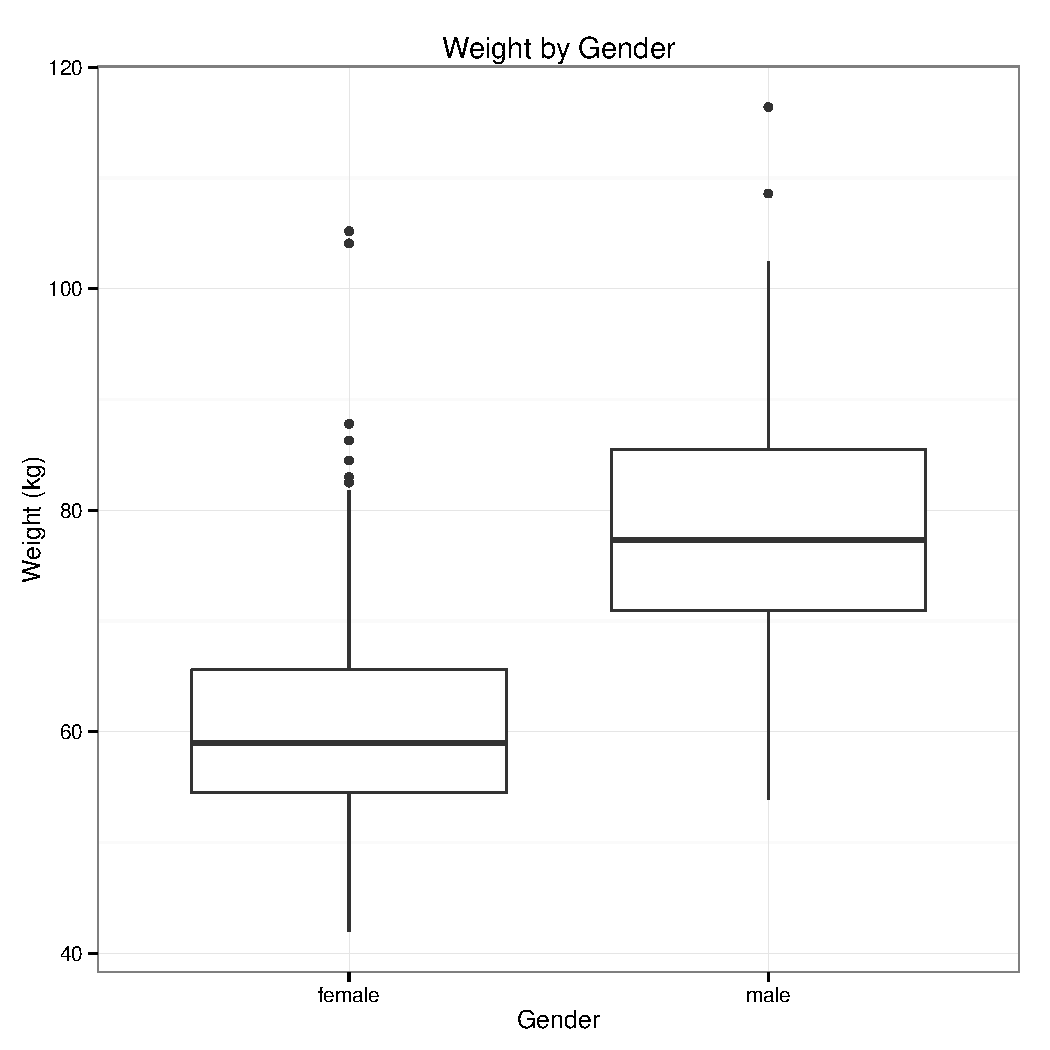
\includegraphics[width=\maxwidth]{figure/weight_plot} 

\end{knitrout}


     \end{column}
     \end{columns}
\end{frame}

%------------------------------------------------

\begin{frame}{Bitrochanteric Diameter and Hip Girth}
     \begin{columns}[t] % contents are top vertically aligned
     \begin{column}[T]{5cm} % each column can also be its own environment
   
{\fontsize{0.275cm}{1em}\selectfont 
Bitrochanteric diameter is the distance between the outer points of the hips and hip girth is the circumference of the hip area measured at the level of the bitrochanteric diameter. The density distributions for both measures are normally distributed (though hip girth is skewed slightly right) and very similar in distribution for both men and women. A scatter plot of hip girth vs. weight suggests that weight increases linerally with increase in hip girth.}

\end{column}
\begin{column}[T]{5cm} % alternative top-align that's better for graphics


\begin{knitrout}
\definecolor{shadecolor}{rgb}{0.969, 0.969, 0.969}\color{fgcolor}
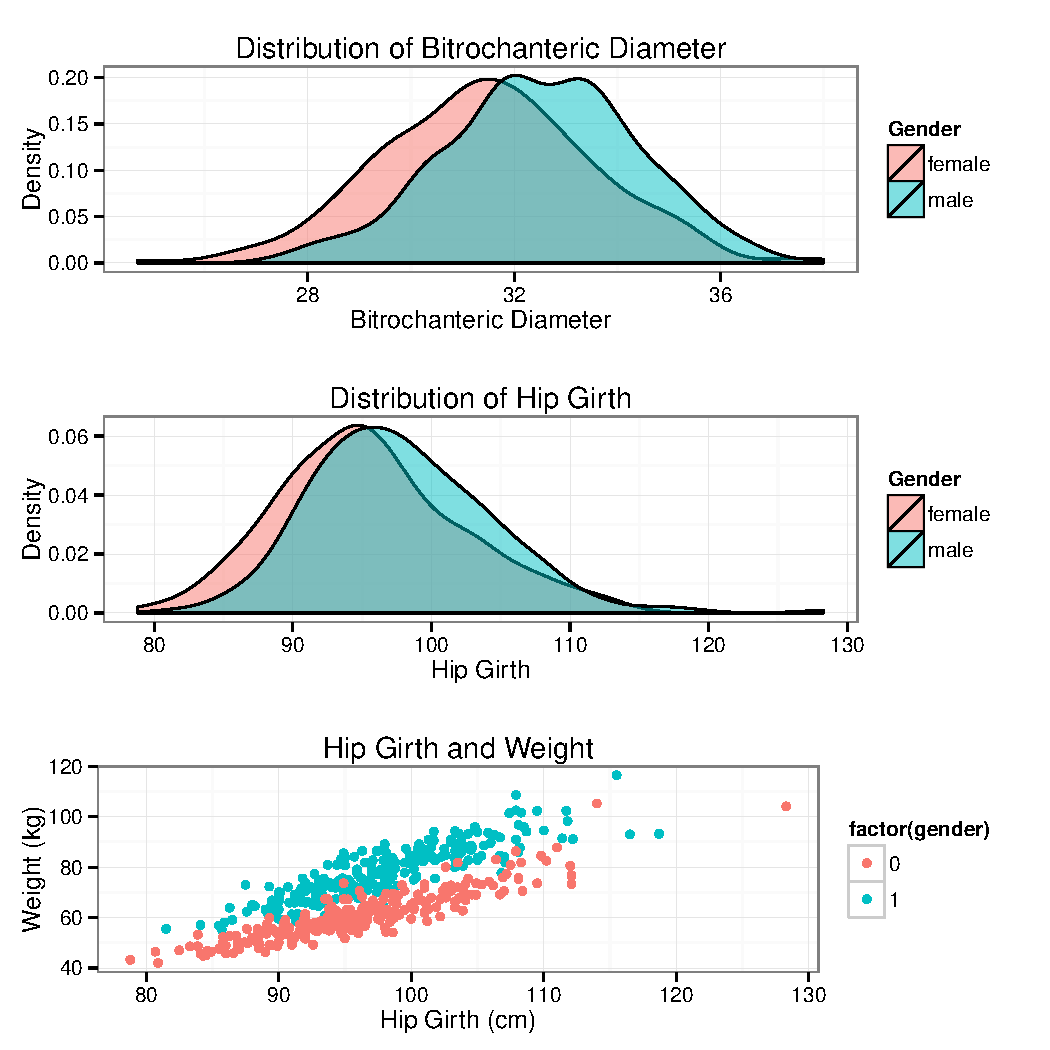
\includegraphics[width=\maxwidth]{figure/hip_plots} 

\end{knitrout}


     \end{column}
     \end{columns}

\end{frame}

%------------------------------------------------

\begin{frame}{Chest and Shoulder}
     \begin{columns}[t] % contents are top vertically aligned
     \begin{column}[T]{5cm} % each column can also be its own environment
   
{\fontsize{0.275cm}{1em}\selectfont 
Chest girth was measured at the nipple line in males and just above breast tissue in females at mid-expiration and shoulder girth was measured over deltoid muscles in both males and females. The density distributions for the two variables are quite similar. Women have narrower, though slightly skeewed, distribution with a much lower mean than that of the men. The scatterplots are also similar in that the regression lines for men and women are nearly identical, indicating that weight increases linearly with increase in shoulder girth, independant of gender.}

\end{column}
\begin{column}[T]{7cm} % alternative top-align that's better for graphics


\begin{knitrout}
\definecolor{shadecolor}{rgb}{0.969, 0.969, 0.969}\color{fgcolor}
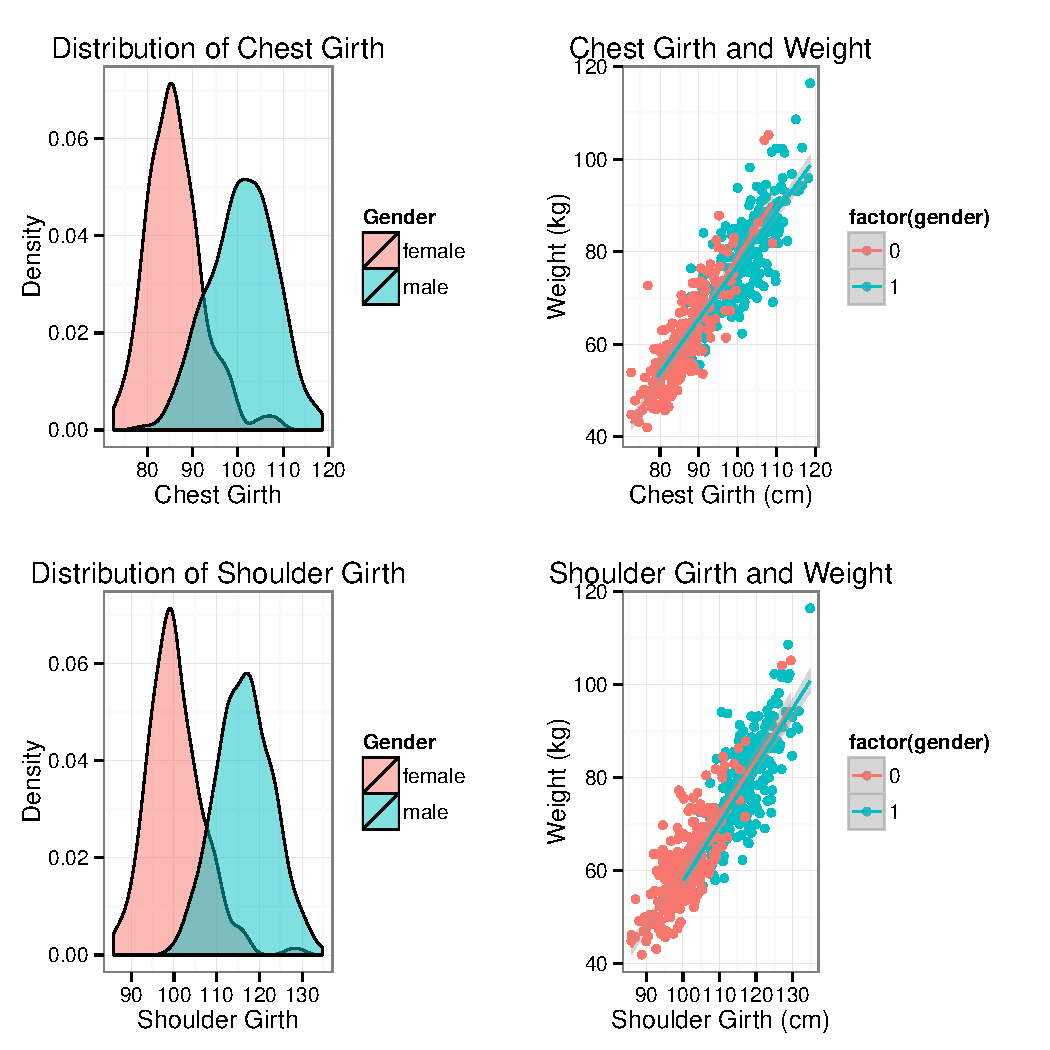
\includegraphics[width=\maxwidth]{figure/chest_plots} 

\end{knitrout}


     \end{column}
     \end{columns}
\end{frame}

%------------------------------------------------

\begin{frame}{Wrist and Navel}
     \begin{columns}[t] % contents are top vertically aligned
     \begin{column}[T]{5cm} % each column can also be its own environment
   
{\fontsize{0.275cm}{1em}\selectfont 
Wrist minimum girth is an average of right and left girths and navel (or abdominal) girth was measured at umbilicus and the iliac crest, using the iliac crest as a landmark. Wrist girth is bimodally distributed, but when divided into male and female, the distributions are normal with some outliers at the high end of the range for females. The distributions for navel girth is normal and remarkably similar for males and females. The scatterplot of navel girth against weight shows a linear relationship with weight increasing with increased naval girth.}

\end{column}
\begin{column}[T]{6cm} % alternative top-align that's better for graphics


\begin{knitrout}
\definecolor{shadecolor}{rgb}{0.969, 0.969, 0.969}\color{fgcolor}
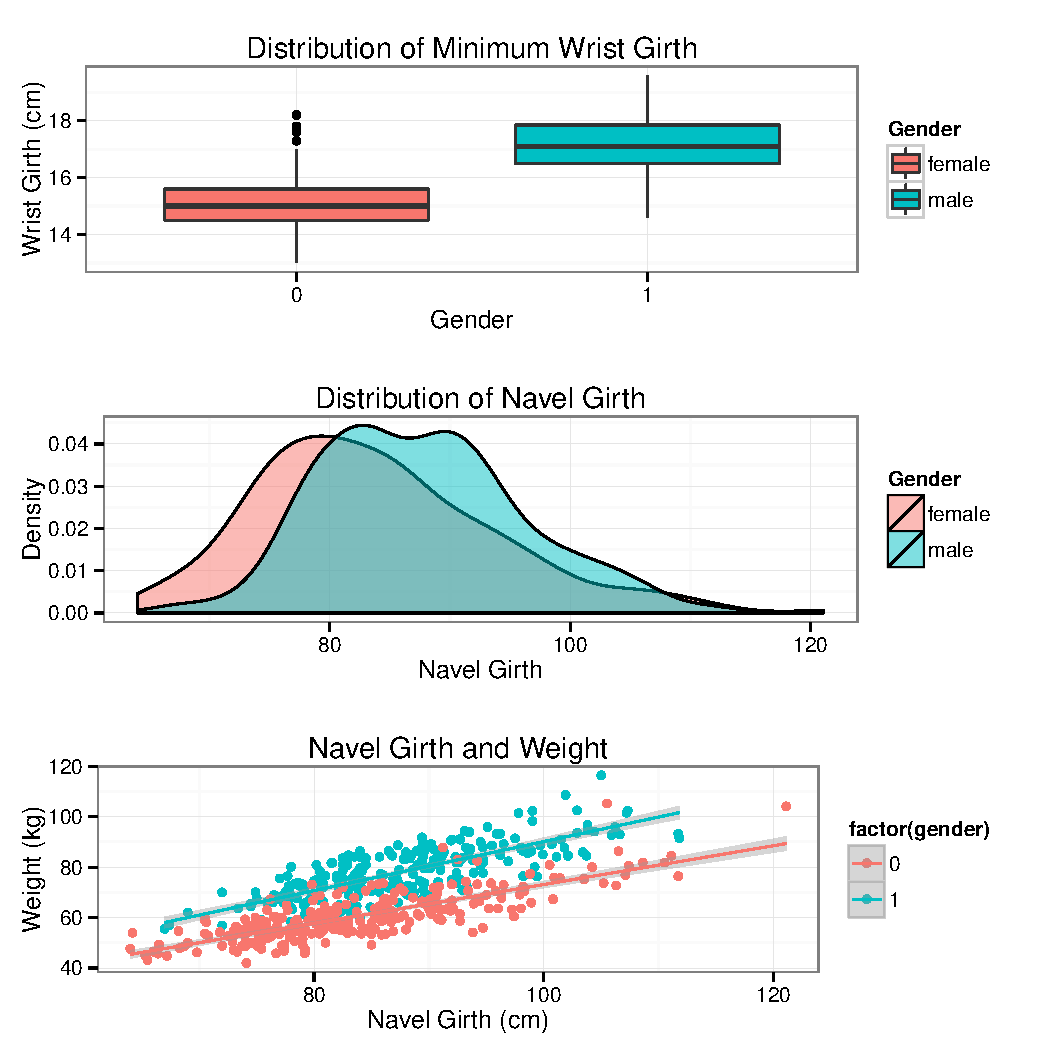
\includegraphics[width=\maxwidth]{figure/navel_plots} 

\end{knitrout}


     \end{column}
     \end{columns}
\end{frame}

%------------------------------------------------

\subsection{Initial Model}

%------------------------------------------------

\begin{frame}{Multiple Linear Regression Model}

Text describing why this model

\begin{block}{Model}
Present predictive model for weight (2) in paper

-fit this model and discuss results

-discuss potential uses for models of this data (finding ideal weight based on skeletal measurements?) and potential problems for applying to whole population (all participants were physically fit)
\end{block}


\end{frame}


%------------------------------------------------

\section{Individual Analysis}

%------------------------------------------------

\subsection{Regression Trees}

%------------------------------------------------

\begin{frame}{Differences between Males and Females (Liza)}
    \begin{columns}[t] % contents are top vertically aligned
     \begin{column}[T]{5cm} % each column can also be its own environment
   
\begin{itemize}
  \item Are there significant differences in the body measurements most useful for predicting weight in males and females?
  \item Is one regression formula appropriate for predicting weight for both genders?
  \item Can we use regression trees to help explore these questions?
\end{itemize}

\end{column}
\begin{column}[T]{7cm} % alternative top-align that's better for graphics


\begin{knitrout}
\definecolor{shadecolor}{rgb}{0.969, 0.969, 0.969}\color{fgcolor}
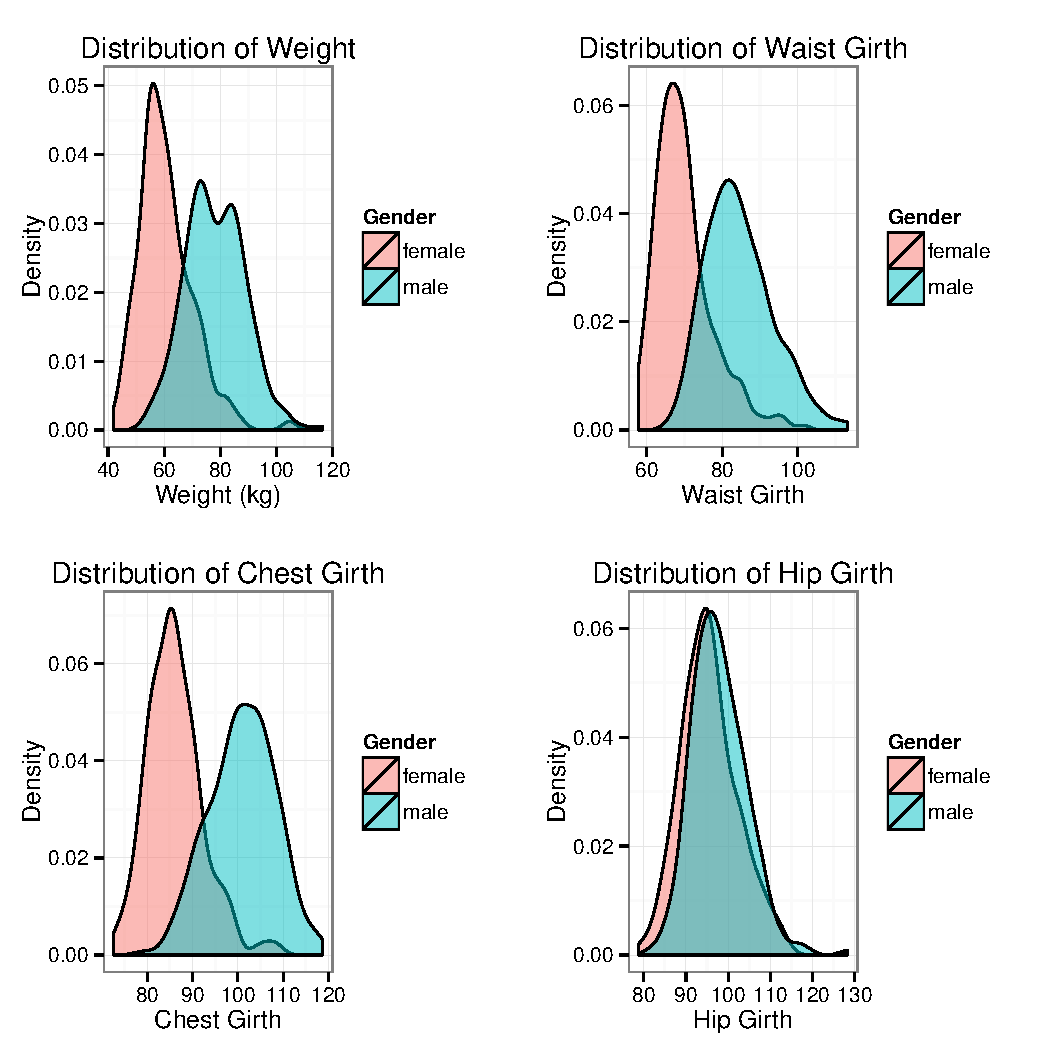
\includegraphics[width=\maxwidth]{figure/gender_plots} 

\end{knitrout}


     \end{column}
     \end{columns}
\end{frame}

%------------------------------------------------

\begin{frame}{Regression Trees}

%this is the set-up for plotting regression trees



%here are the two regression trees. should be side-by-side with some text below.
\begin{knitrout}
\definecolor{shadecolor}{rgb}{0.969, 0.969, 0.969}\color{fgcolor}
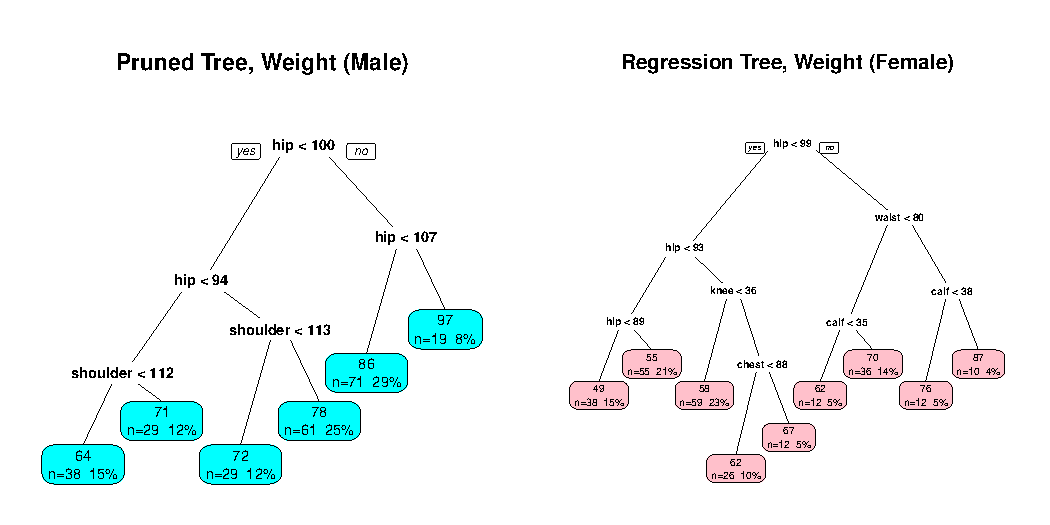
\includegraphics[width=\maxwidth]{figure/mf_plots} 

\end{knitrout}


\begin{itemize}
  \item Variables used in male tree: hip & shoulder girths
  \item Variable used in female tree: hip, knee, chest, waist and calf girths
\end{itemize}

\end{frame}

%------------------------------------------------

\begin{frame}{Conclusions (Liza)}

\begin{itemize}
    \item Regression trees are useful for exploring data and provide a useful alternative to parametric regression methods, though are not intended for making predictions.
  \item Results here suggest that separate models for males and females might be appropriate.
  \item Model fitting and selection exercises could test this hypothesis.
\end{itemize}

\end{frame}
%------------------------------------------------

\subsection{Resampling Inference or something}

%------------------------------------------------

\begin{frame}{Nick}


\end{frame}

%------------------------------------------------
\begin{frame}{Nick}

\end{frame}

%------------------------------------------------

\subsection{Not sure what Yiding decided on}

%------------------------------------------------

\begin{frame}{Yiding}

\end{frame}

%------------------------------------------------

\begin{frame}{Yiding}

\end{frame}

%------------------------------------------------

\subsection{Model Selection}

%------------------------------------------------
\begin{frame}{Emily}

\end{frame}

%------------------------------------------------

\begin{frame}{Emily}

\end{frame}

%----------------------------------------------------------------------------------------

\end{document} 
